\documentclass[english,a4paper,twoside]{ppfcmthesis}

\usepackage[utf8]{inputenc}
\usepackage[OT4]{fontenc}
\usepackage{tabularx}
\usepackage{listings}
\usepackage{enumitem}
\usepackage{lmodern}
\usepackage{booktabs}
\usepackage{float}
\usepackage{placeins}
\usepackage{colortbl}
\usepackage{siunitx}
\usepackage{subcaption}
\usepackage{array}
\usepackage{pgfplotstable}
\usepackage{csvsimple}
\usepackage{hyperref}
\usepackage[algoruled]{algorithm2e}
\usepackage{amsmath}
\usepackage{amsthm}
\usepackage{pdfpages}
\usepackage{xifthen}

% DRAFT
\usepackage{draftwatermark}
\SetWatermarkLightness{0.9}
% END DRAFT

\DeclareGraphicsExtensions{.pdf,.png,.jpg}
% \usepackage{tikz}
% \usetikzlibrary{arrows}
\usepackage{ifthen}

\author{
   Amadeusz Juskowiak \album{106453} \and
   Wioletta Różańska \album{106651}}

\title{Road to solving quadratic assignment problem using Physarum Machines}

\ppsupervisor{Professor~Jacek~Błażewicz}
\ppyear{2016}

\newlength\longest

\lstset{
  basicstyle=\ttfamily\footnotesize, 
  basewidth={0.5em,0.5em}, 
  frame=single, 
  breaklines=true, 
  language=C++
}

\graphicspath{ {figures/} }

%algorithm2e
\SetAlgorithmName{Pseudocode}{List of pseudocodes}

\begin{document}
\graphicspath{{figures/}}
% Front matter starts here
\frontmatter\pagestyle{empty}%
\maketitle\cleardoublepage%

% \includepdf{figures/karta.pdf}
% \cleardoublepage

\pagenumbering{gobble}

\input{"acknowledgements.tex"}
\cleardoublepage
\input{"abstract.tex"}
\cleardoublepage

% Table of contents.
\pagenumbering{Roman}\pagestyle{ppfcmthesis}%
\tableofcontents* \cleardoublepage%

% Main content of your thesis starts here.
\mainmatter%

\chapter{Introduction}
\label{chapter:introduction}

Nowadays, computing science intertwines with various fields of studies posing new challenges for the people of the industry. Every aspect of science is dominated by the technology, just like the everyday lives across the world.

A good example of such interdisciplinary connection is a situation when the companies' managers are required to answer a difficult optimisation question. These businesses mostly are made of different branches, which require transferring of goods between them. Each element of the product could be manufactured in a various departments and is needed in the last part of the assembly in the main office. It could be easier when they produce the whole product in one location, yet seldom it is better to divide the responsibility for specialists in each sector. Although, this process generates som extra costs for the company, it would be crucial to minimise the expenses during assignment of the branches to the locations. Trying to resolve this by hand could be a long process due to the complexity of the problem. However, with usage of computers, it could be answered in a shorter time. The result may not be the optimal one in each case, but it should meet most given assumptions, which is enough to put it into real life usage.

In computer science, this dilemma can be stated as the Quadratic Assignment Problem (QAP).  The QAP is a combinatorial optimisation problem, which was defined by Koopmans and Beckmann in 1957 \cite{koopmans-beckmann1957}, and is a generalisation of an assignment problem. It is NP-hard thus even for small instances finding results is done by approximate methods.

The QAP can be formulated as follows: Given $ n $ different facilities ($F$) and $ n $ different locations ($L$), a weight function $ w: F \times F \mapsto R $ between facilities and a distance function $ d: L \times L \mapsto R $ between locations, find the assignment minimising this cost function:

\begin{equation}
min \sum_{a, b \in F} w(a, b) * d( f(a), f(b))
\end{equation}

Over the years, a number of methods for solving this problem were established. Nevertheless, there is still a place for improvement and experts are searching for new ways of resolving that. Inspired by their works this thesis tries to find an innovative method using living organisms.

The \textit{Physarum polycephalum}, also known as a true slime mould, is a plasmodial organism of yellow colour. Its single cell body is considered to be the biggest in the world \cite{stephenson1994myxomycetes}. Taking into account the current state of classification, it belongs to the Kingdom Protista, however, this used to frequently change due to the fact that it does not exactly match any of the recognised kingdoms. The \textit{Physarum polycephalum} move very slowly, in a branching pattern as it forages for new food sources. It ingests bacteria, fungal spores and during the experiments --- oatmeals.

\section{Motivation}
\label{section:introduction_motivation}


\section{Goal}
\label{section:introduction_goal}

This thesis presents the road to solving Quadratic Assignment Problem (QAP) based on behaviour of Physarum machines.
Deep analysis of each part of the main dilemma is essential to proceed with future works.

The first task is to carry out the detailed investigation of the behaviour and capabilities of the slime mould. Without the understanding of organisms, it is not possible to replicate its operations. For this purpose, the living plasmodia will be observed, giving us details of the schemes of the movement when looking for food. This will be studied in order to extract similar patterns and facilitate the creation of
calculation method based on them, which could be transported into the computer environment. We will implement such plasmodial behaviour for solving QAP.

Furthermore, not only the direct observation of \textit{Physarum polycephalum} behavior is needed here, but also a careful examination of previous studies. Such research will also give as a thorough look into behaviour and abilities of the slime mould, especially taking into account the possibility of using our model algorithm as an inspiration for solving computational problems.

Next, the analysis of the research related to the QAP in general will be conducted, leading to better understanding of the problem and showing the current practices for solving it. Recognising the dilemma will make it easier to fit the algorithm based on slime moulds to the QAP.

The key element of this thesis is to apply methods used by \textit{Physarum polycephalum} for solving QAP. This step will consist of adaptation of the biological mechanisms, implementation of simulation and analysis of the results. In this way, we connect the previously acquired theoretical knowledge and a practical task. And last, but not least, our aim will be to create the innovative method for solving QAP.


\section{Chapters}
\label{section:introduction_chapters}

The thesis is divided into five chapters and includes one appendix.

\begin{itemize}  
\item Chapter two describes the physarum organisms characteristics such as a position in the hierarchy, basic information about the species, basics of operations, emerging behavior and previous research.
\item Chapter three outlines the quadratic assignment problem (QAP). It consists of a different interpretation, practical usages, current exact solution and current heuristic. 
\item Chapter four presents the algorithm, which will be proposed as the result of this thesis. It will be a pseudophysarum machine providing working metaheuristics based on observed behavior.
\item Chapter five summarizes the research and is focusing on future work ideas.
\item Appendix A includes description of hardware-software platform, which is used for examination of physarum.
\end{itemize}

\section*{Work Distribution}
\label{section:introduction_distribution}

The work was distributed between two coworkers in a manner described below:
\begin{itemize}
  \item Amadeusz Juskowiak conducted a research about Physarum Polycephalum and he observed the behavior of alive organisms. He also designed and implemented the algorithm approximating QAP.
  \item Wioletta Różańska conducted a research about quadratic assignment problem. She also implemented the algorithm approximating QAP and carried out comparative tests with existing solutions.
\end{itemize}

Next to these tasks both authors wrote the text of this thesis.



\chapter{Background}
\label{chapter:background}

Thorough research of both \textit{Physarum polycephalum} and \textit{Quadratic Assignment Problem} has been conducted. Principles and related works for both fields are presented in following subsections. Obtained knowledge is the ground and an inspiration for a design of solution proposed in a next chapter.


\section{\textit{Physarum polycephalum}}
\label{section:background_physarum}

The organism being a subject for this work is \textit{Physarum polycephalum} also called the many-headed slime mould. It is a member of the \textit{Physaridae} family of slime moulds, in order of \textit{Physarales}, class \textit{Myxogastria}, phylum \textit{Myxomycete}, supergroup \textit{Amoebozoa} in \textit{Protista} kingdom. While current position in taxology is well defined, presented characteristics should justify why scientists used to have problems with classification of the Physarum \cite{stephenson1994myxomycetes}.

In order to make the thesis readable, terms \textit{Physarum polycephalum}, \textit{Physarum} or \textit{the slime mould} will be used interchangeably as the subject is unambiguously defined. As none of the authors have a background in biology, concepts are presented from a computer scientist's perspective in minimal, yet exhaustive, form.


\subsection{Biological characteristics}

\textit{Physarum polycephalum} is a very peculiar organism. Even it is a \textit{Protista}, which are usually very small, it can be observed with a naked eye --- it is one among the biggest currently known unicellular organisms \cite{stephenson1994myxomycetes}. In its natural habitat, under cool, dark and humid conditions the slime mould exists in form of a yellow semistructurised blob (as seen in figure \ref{figure:bp_habitat}). Its occurrence is fairly common around the globe, however species \textit{Physarum polycephalum} does not occur naturally in Poland \cite{narkiewicz2013grzyby}. It feeds on bacteria, fungi and other sources of basic nutrients (such as aminoacids and carbohydrates).

In laboratory conditions, \textit{Physarum} is stored on Petri dishes filled with a non-nutritious agar (figure \ref{figure:bp_petri}). The agar base provides humid environment required for supporting plasmodial stage of the slime mould. A sterile oatmeal or even a soft porridge is used as a controlled source of nutrients. The complete description of a storage and an observation protocol, among other information, is provided in Appendix \ref{chapter:protocol}.

\begin{figure}
  \centering
  \begin{subfigure}{0.45\textwidth}
    \centering
    \includegraphics[width=0.9\textwidth]{background/physarum/habitat.jpg}
    \caption{Natural habitat (image source: flickr.com/randomtruth)}
    \label{figure:bp_habitat}
  \end{subfigure}
  \begin{subfigure}{0.45\textwidth}
    \centering
    \includegraphics[width=0.9\textwidth]{physarum/IMG_1194.jpg}
    \caption{Petri dish}
    \label{figure:bp_petri}
  \end{subfigure}
  \caption{\textit{Physarum polycephalum} in plasmodial stage}
\end{figure}

\begin{figure}
  \centering
  \includegraphics[width=0.94\textwidth]{background/physarum/lifecycle.png}
  \caption{Life cycle of \textit{Physarum polycephalum} (image source: Carolina Biological Supply)}
  \label{figure:bp_lifecycle}
\end{figure}

As representant of \textit{Myxomycete}, a life cycle of the slime mould is very complex, including haploid and diploid phases (as seen in figure \ref{figure:bp_lifecycle}). Such cycle is a result of an evolutionary adaptation \cite{stephenson1994myxomycetes}. Formation of the diploid sporangium occurs as a result of worsening conditions (such as inadequate temperature, humidity or acidity). Sporangium releases spores, which can germinate into ameboid swarm cells. Such cell can enclose into a cyst to protect itself, until environmental conditions improve. When conditions are favourable, the amoeboid cell turns into a flagellated swarm cell. Swarm cells can merge, fuse their nuclei and start mitotic process resulting in a formation of a plasmodium \cite{jones2015pattern}.

For purposes of unconventional computing applications, \textit{Physarum} is preferred in its plasmodial stage. However, during the research transformations into other states are inevitable and must be dealt with. In case of drying or an enforced starvation, sclerotium is formed --- in this dormant phase \textit{Physarum polycephalum} can survive for many years until dampness and nutrients are provided again. Plasmodium forms protoplasmic tubes (also called pseudopodia) as a response to food availability. Such tubes are used for a discovery and transportation of nutrients. The tubes are built in similar way to animal muscles. The ectoplasm contains actin and myosin complexes, which are organised into regular structures that form tubes. Such actomyosin complexes generate a contractile motion which results in streaming of the protoplasm. Furthermore, synchronised oscillations of directions of protoplasm streams can be observed. Nutrients are transported at first in one direction, and after 1-2~minutes the direction is reversed. Period of this oscillation depends on the environment quality and an accessibility of food \cite{wohlfarth1979oscillatory} --- higher frequency oscillations are generated where nutrients are available and favourable environment exist, low frequency oscillations are caused by lack of food or as a result of harmful conditions. 

The plasmodium can grow around 10~mm per hour when it actively explores the environment \cite{coggin1996dynamic}. While moving, plasmodium leaves polysaccharide traces (informally called slime, hence the name slime mould). The network of the protoplasmic tubes adapts, forming efficient ways of transporting nutrients, depending on their amount and quality \cite{nakagaki2004obtaining}. Exploiting this behaviour is a fundamental principle for building physarum machines.


\subsection{Related works}

Since early 1960s \textit{Physarum polycephalum} has been a subject to many biological and microbiological studies \cite{guttes1964mitotic,daniel1962method}, however it is late 70s when its computational-like behaviours have been observed \cite{wohlfarth1979oscillatory}. Research towards computational applications of the \textit{Physarum} truly started in 1990s. Nowadays, there exist two prominent research centres focusing on the slime mould --- one based in United Kingdom (Andrew Adamatzky\footnote{~\url{http://uncomp.uwe.ac.uk/adamatzky/}}, Jeff Jones\footnote{~\url{http://uncomp.uwe.ac.uk/jeff/}} from University of West England, Bristol), second in Japan (Toshiyuki Nakagaki\footnote{~\url{http://www.cris.hokudai.ac.jp/cris/en/research/ob/ob\_innovative/nakagaki.html}}, Hokkaido University, Sapporo). Some of their works excited us about slime mould capabilities and inspired to write this thesis \cite{nakagaki2000intelligence,adamatzky2010physarum,jones2015pattern,adamatzky2007physarum}. Experiments presented here focus on different aspects of \textit{Physarums} behaviour. Understanding them gives impression of emerging computational power of such simple organism as a slime mould.


\subsubsection{Maze-solving capabilities}

Maze-solving or a more constricted problem of finding, preferably shortest, paths is very common in practice. It has many applications and many possible algorithms are already available. Algorithms such as breadth-first search or more complex $A*$ are commonly used for solving mazes \cite{zelkowitz1979principles}. However Toshiyuki Nakagaki et al. proposed usage of slime moulds' natural capabilities as an unconventional solution to this problem \cite{nakagaki2000intelligence}.

In order to use \textit{Physarum} to solve a labyrinth, a maze must be represented as a physical object. Such maze is modelled on a Petri dish where floor is made of non-nutrient agar and walls are made of thin plastic film (the maze used in the experiment is presented on figure \ref{figure:bp_maze_initial}). As the slime mould strictly prefers humid environment of the agar it will not pass arid walls made of plastic film. 

\begin{figure}
  \centering
  \begin{subfigure}{0.45\textwidth}
    \centering
    \includegraphics[width=0.9\textwidth]{background/physarum/maze1.jpg}
    \caption{Plasmodium initially filling maze}
    \label{figure:bp_maze_initial}
  \end{subfigure}
  \begin{subfigure}{0.45\textwidth}
    \centering
    \includegraphics[width=0.9\textwidth]{background/physarum/maze2.jpg}
    \caption{Intermediate state}
    \label{figure:bp_maze_intermediate}
  \end{subfigure}
  \begin{subfigure}{0.45\textwidth}
    \centering
    \includegraphics[width=0.9\textwidth]{background/physarum/maze3.jpg}
    \caption{Final route}
    \label{figure:bp_maze_final}
  \end{subfigure}
  \caption{\textit{Physarum} in various states of the maze experiment \cite{nakagaki2000intelligence}}
\end{figure}

There are four possible routes available $\{(\alpha_1,\beta_1), (\alpha_1,\beta_2), (\alpha_2,\beta_1), (\alpha_2,\beta_2)\}$ between entry point $A$ and exit point $B$. The oatmeal-agar-based source of nutrients is planted in both, entry and exit points, while large enough plasmodium is placed over whole floor of the maze. As time passes it can be observed that plasmodium retracts its body from labyrinth's dead-ends, leaving traces of slime where it previously has been placed (figure \ref{figure:bp_maze_intermediate}). 

As a result the slime mould rests only on direct paths connecting the entry with an exit point (figure \ref{figure:bp_maze_final}). Furthermore, it has been observed that \textit{Physarum polycephalum} usually prefers shortest $(\alpha_2,\beta_1)$ path as it prefers most efficient way for transferring nutrients. While obtained results are satisfactory, it must be noted that the whole process takes about 4~hours. 


\subsubsection{Spatial memory}

Memory is usually associated with neurological functions of brain, however it can be externalised in multiple ways, in example as pheromone trails of ants \cite{carroll1973ecology} or even notes-writing as humans do \cite{fisher1973effect}. Team of researchers from University of Sydney, demonstrated that \textit{Physarum polycephalum} uses its slime as a form of spatial externalised memory \cite{reid2012slime}.

A common problem testing autonomous navigational skills in robotics is the U-shaped trap problem \cite{chatterjee2001use}. An efficient solution of this issue requires some kind of a spatial memory or other navigational aids \cite{balch1993avoiding}, therefore it was a good candidate for a test of slime mould's memorising capabilities. The U-maze problem requires an agent (a robot or as in this example the slime mould) to navigate itself from starting position to the goal, where goal is hidden beside the U-shaped trap (figure \ref{figure:bp_trap_model}). The agent has to use some kind of environment map or use a reactive guidance to bypass the trap (figure \ref{figure:bp_trap_model_success}), otherwise, most probably it will be stuck inside the trap (figure \ref{figure:bp_trap_model_failure}).

\begin{figure}
  \centering
  \begin{subfigure}{0.33\textwidth}
    \centering
    \includegraphics[width=0.9\textwidth]{background/physarum/trap_initial.eps}
    \caption{Initial setup}
    \label{figure:bp_trap_model}
  \end{subfigure}
  \begin{subfigure}{0.37\textwidth}
    \centering
    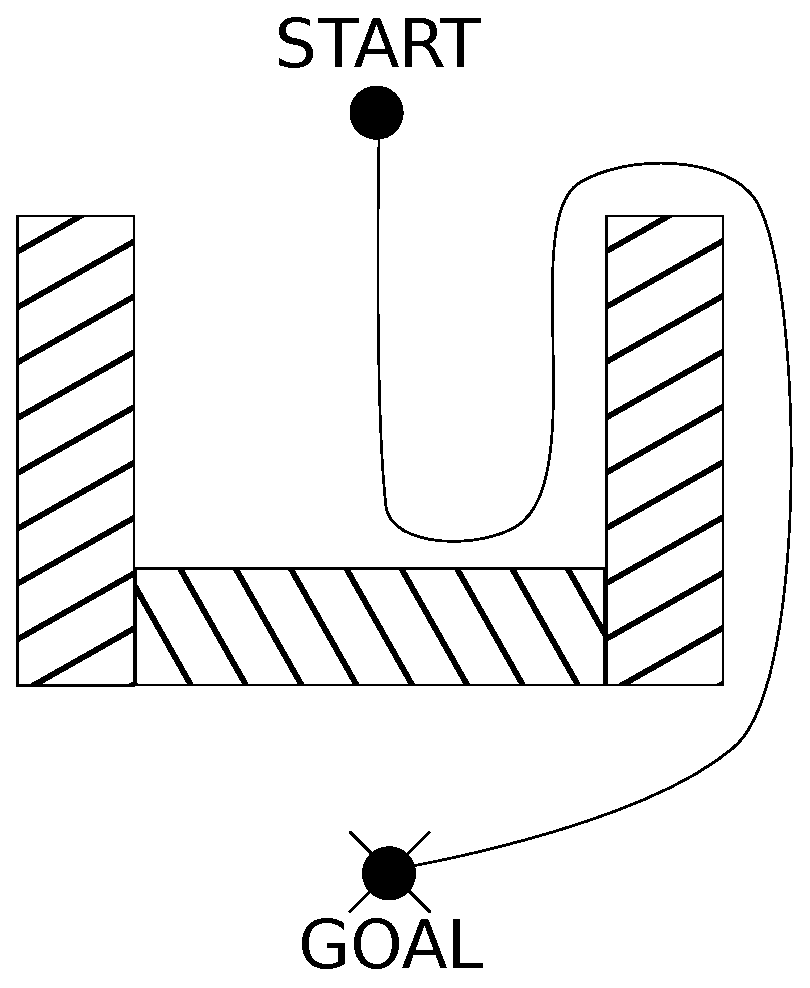
\includegraphics[width=0.9\textwidth]{background/physarum/trap_success.eps}
    \caption{Example successful route to goal}
    \label{figure:bp_trap_model_success}
  \end{subfigure}
  \begin{subfigure}{0.37\textwidth}
    \centering
    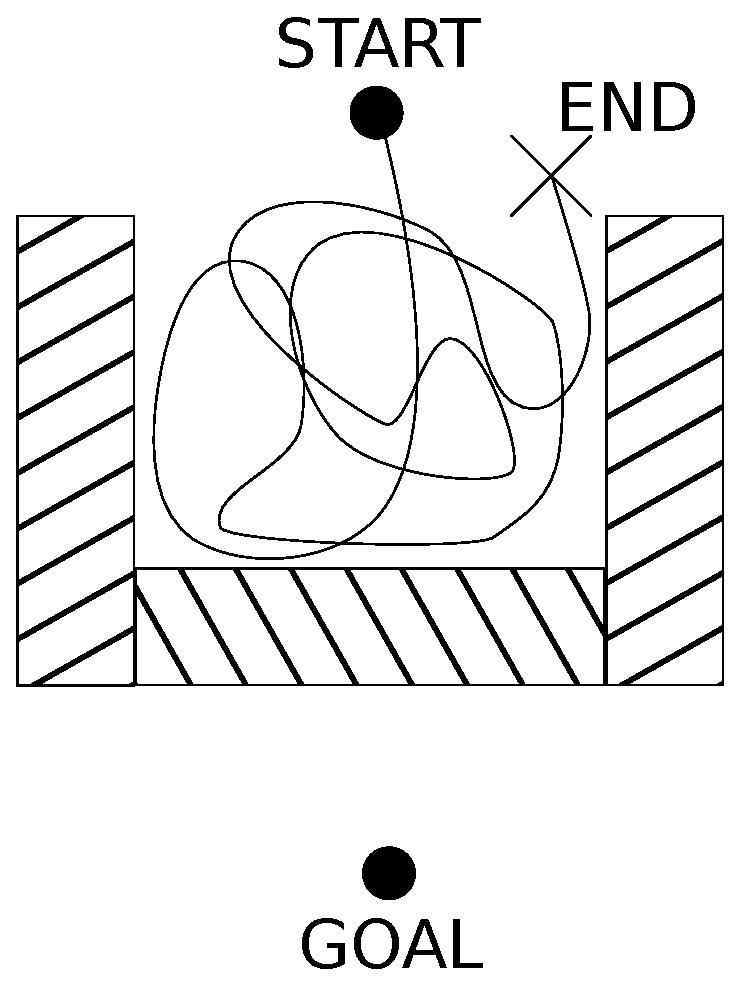
\includegraphics[width=0.9\textwidth]{background/physarum/trap_failure.eps}
    \caption{Typical failure}
    \label{figure:bp_trap_model_failure}
  \end{subfigure}
  \caption{U-trap test with possible outcomes}
\end{figure}

The experiment conducted by Reid, Latty, Dussutour and Beekman \cite{reid2012slime} used \textit{Physarum polycephalum} as an agent in the non-nutrient agar environment, where the trap was made out of acetate and the goal was a highly nutritious glucose. The agar base allows diffusion of glucose particles, creating nutrients gradient towards the goal. Initial experiments indicated that \textit{Physarum} moves in a direction where its slime is not present, however if no such direction exists (there is the slime all around plasmodium) it moves in random direction or all over the substrate. Therefore a slime mould has a choice to explore unexplored, however it is not an ultimate one, as it always can maneuver in previously visited areas. 

\begin{figure}
  \centering
  \includegraphics[width=0.74\textwidth]{background/physarum/trap_experiment.jpg}
  \caption{\textit{Physarum polycephalum} in U-trap experiment on a slime covered substrate \cite{reid2012slime}}
  \label{figure:bp_trap_experiment}
\end{figure}

As the slime is a stable nonliving substance, mostly made of galactose polymers it can be easily handled, collected and replanted \cite{mccormick1970isolation}. Two kinds of the experiment have been designed --- in a first one, previously collected slime is placed all over the substrate (figure \ref{figure:bp_trap_experiment}), while in a second one the substrate is just a clean agar. The first environment constrains \textit{Physarum} not to rely on slime for navigation (as implanted slime acts as noise), unlike the second one, in which \textit{Physarum} can use the slime freely for its navigation.

Experiments have shown that \textit{Physarum} placed on a substrate already coated with the slime cannot easily escape out of the U-trap --- it spends there a long time until it leaves the trap. Furthermore, only in 33\% of 24 repeated cases plasmodium reaches the goal. However, when plasmodium is put on a clean agar substrate, an ability to use its slime as the navigational aid results in reaching the goal in 96\% of cases. Both, travelled distance and time to reach the goal, were much shorter when the organism were able to use the slime. These findings prove that \textit{Physarum polycephalum} can sense its extra-cellular slime and uses its existence as a form of an externalised spatial memory for a recognition of previously explored areas.


\subsubsection{Adaptive network design}

Networks are used in a various fields of engineering --- from civil roads, water pipelines, railway systems to energy grids, not to mention the Internet. Design of a practical robust network usually implies a balance between efficiency, cost and fault tolerance. Increasing robustness involves a creation of redundant connections between some of the nodes. This might seem not to be profitable, however it allows the network to gracefully degrade and still maintain some of its throughput. Japanese team of scientists showed that \textit{Physarum polycephalum} can be used to design networks on a par with human or algorithmic designs \cite{tero2010rules}.

% TODO remove letters from pictures
\begin{figure}
  \centering
  \begin{subfigure}{0.33\textwidth}
    \centering
    \includegraphics[width=0.9\textwidth]{background/physarum/network_initial.jpg}
    \caption{Initial placement}
    \label{figure:bp_network_initial}
  \end{subfigure}
  \begin{subfigure}{0.33\textwidth}
    \centering
    \includegraphics[width=0.9\textwidth]{background/physarum/network_intermediate_a.jpg}
    \caption{State in $t=8h$}
    \label{figure:bp_network_intermediate_a}
  \end{subfigure}
  \\
  \begin{subfigure}{0.33\textwidth}
    \centering
    \includegraphics[width=0.9\textwidth]{background/physarum/network_intermediate_b.jpg}
    \caption{State in $t=16h$}
    \label{figure:bp_network_intermediate_b}
  \end{subfigure}
  \begin{subfigure}{0.33\textwidth}
    \centering
    \includegraphics[width=0.9\textwidth]{background/physarum/network_final.jpg}
    \caption{Final plasmodium state}
    \label{figure:bp_network_final}
  \end{subfigure}
  \caption{Example \textit{Physarum polycephalum} network in railway experiment \cite{tero2010rules}}
\end{figure}

The choice of the slime mould was quite natural: the organism forms a network as it forages and it can be assumed, that through many years of evolution, its designs has reached an equilibrium between cost, efficiency and robustness. The researchers prepared an experiment based on design of Tokyo-area rail network. On a substrate made of an agar, thirty~six~food~sources (identical oat meals) have been placed, resembling a real topographical positions of the rail stations (figure \ref{figure:bp_network_initial}). A blob of plasmodium has been placed where city of Tokyo would be, after some time, as the slime mould forages, it covered the substrate and connected each food source (figures \ref{figure:bp_network_intermediate_a}, \ref{figure:bp_network_intermediate_b}). Afterwards \textit{Physarum} retracted its body from the empty areas, leaving only interconnected food sources (figure \ref{figure:bp_network_final}). It should be observed, that some junctions have been left where no food is placed --- these are Steiner~points \cite{kou1981fast} enhancing overall efficiency of the network.

The experiment has been replicated 20~times, each time resulting in slightly different design of the final network, however it always resembled the Tokyo rail network designed by civil engineers. In order to even further improve similarity, the substrate has been illuminated where geographical features restrain the rail network. As the slime mould avoids light, such illumination acted as a constraint for the network --- these networks bore even bigger similarities to original plans than networks made without constraints. 

In the end, it was concluded that networks designed by \textit{Physarum polycephalum} have lower overall cost with similar transport efficiency, however they lack a bit of fault tolerance --- while in only 4\% of faults the real rail network would lead to isolation of any part, in case of networks designed by the slime mould such isolation would occur in 14\% of faults. Still, these results are acceptable as \textit{Physarum}'s network designs have much lower cost. Nonetheless, it should be noted that these networks should not be compared directly --- stops on Tokyo network have not been planned at once, they evolved as the city grew, unlike the task given to \textit{Physarum} which assumed knowledge of stops locations. The processes differs even more, as design of a real rail network is usually centralised, however the slime mould acts as a self-organised mechanism without the central control.


\subsubsection{Slime mould models}

In the same work \cite{tero2010rules}, Japanese researchers proposed a mathematical model of \textit{Physarum polycephalum} used for adaptive network designs based on a flow network. The slime mould has been adapted as initially random lattice, where edges represents the pseudopodia. The flux inside pseudopodia has been accurately defined with Hagen-Poiseuille formula for the laminar flow \cite{sutera1993history}. The simulation is conducted in discrete time steps. In each step a random food source node is selected to drive the flow through the network, where another food source is selected to be a sink. Strength of the flow influences conductivity of each tube --- unused tubes gradually disappear, while effective tubes adapt to increase throughput. This model reflects some of the properties of the real slime mould and can be used for design of adaptive network model.

Quite profound work on modelling \textit{Physarum polycephalum} has been presented by Jeff Jones in his book \cite{jones2015pattern}. He modelled plasmodium in a multi-agent fashion as a material made of multiple particles working towards a reaction-diffusion process. A single agent represents a particle of plasmodium gel/sol structure --- its movement resembles protoplasmic flow, however when it is immobile, it could be treated as the gel matrix. Each agent can sense chemoattractants in the two-dimensional substrate using three forward-directed sensors. A single agent can move in oscillatory or non-oscillatory modes. First one can be used to approximate resistance within plasmodium and the second one represents an ideal movement without any external forces. Plasmodium-like behaviour emerges from the collection of such randomly placed agents. Furthermore chemoattractants and chemorepellents can be placed on the substrate, stimulating the agents to regroup and move. This model can be tuned to closely resemble real \textit{Physarum polycephalum} in a variety of environment conditions.

% TODO crop images so they are aligned
\begin{figure}
  \centering
  \begin{subfigure}{0.3\textwidth}
    \centering
    \includegraphics[width=0.9\textwidth]{background/physarum/tsp_initial.png}
    \caption{Initial placement within convex hull}
    \label{figure:bp_tsp_initial}
  \end{subfigure}
  \begin{subfigure}{0.3\textwidth}
    \centering
    \includegraphics[width=0.9\textwidth]{background/physarum/tsp_intermediate.png}
    \caption{State after removal of some agents}
    \label{figure:bp_tsp_intermediate}
  \end{subfigure}
  \begin{subfigure}{0.3\textwidth}
    \centering
    \includegraphics[width=0.9\textwidth]{background/physarum/tsp_final.png}
    \caption{Final state of simulation}
    \label{figure:bp_tsp_final}
  \end{subfigure}
  \caption{Solving TSP using shrinking blob method \cite{jones2014computation}}
\end{figure}

\begin{figure}
  \centering
  \includegraphics[width=0.3\textwidth]{background/physarum/tsp_readout.png}
  \caption{TSP tour readout method \cite{jones2014computation}}
  \label{figure:bp_tsp_readout}
\end{figure}

Based on this model Jeff Jones and Andy Adamatzky proposed a method of a shrinking blob for approximating solution of Travelling Salesman Problem (TSP) \cite{jones2014computation}. This method requires putting previously described agents inside a convex hull computed on topology of TSP input (figure \ref{figure:bp_tsp_initial}). Initially chemoattractants are placed nearby data points. As simulation goes some agents are removed from the virtual plasmodium, effectively shrinking the blob (figure \ref{figure:bp_tsp_intermediate}). Simulation is stopped when each node is partially uncovered --- a $5 \times 5$ window passes over each node and checks for such condition (figure \ref{figure:bp_tsp_final}). Resulting TSP tour can be read by tracking perimeter of the blob at the end of simulation (figure \ref{figure:bp_tsp_readout}). The authors evaluated this method to be 4.27\% worse than the optimal solutions in their dataset.


\subsection{Observations}
\label{ss:obervations}

Using the financial support from Poznan University of Technology, we obtained the culture of \textit{Physarum polycephalum} from Carolina Biological Supply. The access to the living organism allowed us to observe its behaviour in a variety of conditions. As for computer scientists, who have no experience in wet lab works, it was a very challenging task to handle alive slime mould, yet very educative one --- detailed methods of handling the organism are presented in Appendix \ref{chapter:protocol}.

We usually worked with the slime mould on a 2\% non-nutrient agar substrate, however two other substrates have been tested: a wet towel and an aluminium foil. We have placed plasmodium on dampened kitchen towel, as we believed that it is easier to manage than the agar solution. As for the wet towel, no mobility has been affected, however water evaporated quickly and regular moisturising has been required. Furthermore moving the colony out of the kitchen towel was more complicated, as it was difficult to cleanly separate the organism from the substrate. In the case of aluminium foil as the substrate, while it makes the separation easy it was not used for long, as this substrate lacks ability to bound water, which is required for keeping \textit{Physarum polycephalum} in its plasmodial stage. A standard non-nutrient agar keeps moisture for a long time (up to 10 days until the plasmodium is moved to new substrate) and keeps smooth surface if properly poured into Petri dish, making it quite easy to relocate the colony. Agar gel-like structure prohibits \textit{Physarum} from escapades to the bottom part of Petri dish, unlike porous kitchen towel. 

We used a classic oatmeal as primary food for the slime mould. It is composed primarily of starch, some proteins, little fat and trace amount of sugar. We usually used oats as a whole or smaller distinct pieces, but for better precision a sterile porridge paste has been used. Nutrients available in oatmeal made the plasmodium move with 9--10~mm/hr (measured on frontier). We experimented with use of table sugar as nutrient, resulting in 8~mm/hr velocity and decolorisation of the plasmodium. Usage of syrup made of pure glucose made the subject to move relatively fast 12--16~mm/hr, however it was completely decolorised and no networking behaviour was observed. It is possible that glucose has dissolved within an agar substrate changing the slime mould's foraging strategy to the simpler one --- no need to look for food as the substrate became source of nutrients. We also confirmed that valerian drops made from valerian root act as strong chemoattractant for the slime mould \cite{adamatzky2012physarum} --- given choice of oatmeal and oatmeal mixed with valerian drops \textit{Physarum} foraged towards the second one in ten of ten cases. Additionally, when multiple sources of food, varying in their size, were introduced to a slime mould, it always ended up foraging on the largest one. In the end we reaffirmed that oatmeals are preferred source of nutrients for laboratory use. As for water, distilled water was used, however when no access to such pure water was possible a tap water has been used. We observed that tap water slightly decreased \textit{Physarum} mobility to abound 8-9~mm/hr, with no other consequences --- it could be caused by chlorine or fluorine used for tap water disinfection \cite{uden1983chlorinated}.

The culture of \textit{Physarum polycephalum} has been kept in dark shoebox as these conditions are favourable for growth of plasmodium \cite{adamatzky2010physarum}. When the slime mould has been kept in a window-lit room, plasmodium growth has been massively reduced (none to as little as 4~mm/hr). However we found that infrared light (near-IR LED has been used) made no observable effects on the plasmodium --- one can use infrared light and infrared camera to observe plasmodium as it forages in the dark. We assume that infrared light carries so little energy, so it makes no harm to the organism. When the Petri dish has been partly lit with visible light \textit{Physarum} strongly avoided bright areas --- it stayed at most 5~mm close to the light patch (as some light has been diffused within agar substrate). A green laser (20~mW power, 520~nm wavelength) has been used with similar results, however the area was lit more precisely. 

Pattern of light can be used to create constraints for the plasmodium --- arrangement of LEDs or lasers can be used for precise limits, some even propose usage of gobo lights or projectors for complex patterns \cite{zhu2013amoeba}. Constraints can be also made using physical or chemical methods. We tested table salt and easily obtainable citric acid as potential chemorepellents. A line made of table salt became an obstacle for crawling plasmodium, it never crossed this line, instead the slime mould bypassed around such obstacle. Same effects have been observed with the citric acid crystals, furthermore enclosing the slime mould within a circle made of citric acid effectively reduced its foraging area to within the circle. While chemical repellents are effective, in a longer term they dissolve into agar substrate, contaminating it and making it unsuitable for keeping the subject alive. Physical based obstacles can be a solution to this problem. We tested two solutions --- removal of agar substrate and addition of thin plastic sheet. Both methods exploit the fact that \textit{Physarum} requires a wet substrate to keep its active plasmodial stage, thus it avoids dry areas. The first method requires cutting out some of the agar resulting in exposing dry area of the Petri dish, where the second one requires cutting pieces of plastic (we used thin yet hard polypropylene foil) and putting them on a top of the substrate creating a dry area. Both methods are \textit{de facto} effective, however we observed unlikely cases (2 out of 10 experiments) where plasmodium has crossed such physical barrier. This observation can be compared to behaviour of an electrical current, which follows path of least resistance, but if insulator is not thick enough it actually can be bypassed --- indeed, usage of thicker physical barriers makes them more robust. 

Hereafter we can conclude that creating barriers is a tradeoff between side~effects and complexity:
\begin{itemize}
  \item light-based --- have no side effects, but are complex to create,
  \item chemical --- easy to create, but with catastrophic long-term effect,
  \item physical --- moderate to create, but somehow unreliable, occupying large area.
\end{itemize}

% TODO add image
The slime mould fed with oatmeal on an agar substrate forages in network structure. Individual oatmeals are connected by pseudopodia varying in thickness. Width of protoplasmatic tubes is proportional to nutrients transported with the flux between nodes of the plasmodium. The organism created many nodes where no food have been placed, thus optimising paths for the nutrients. Moreover during experiments with various food sources and barriers, regular changes in width of the tubes have been observed as response to the local environment. The pseudopodia thickness changed up to 20\% over time span of 60-170~seconds --- frequency of such oscillation has been greater near positive stimulus (food source), lower frequencies have been observed in tubes closer to chemorepellents (such as salt). This behaviour can be used as a form of communication between \textit{Physarum} and other devices --- a time-lapse imaging can be used to acquire such reaction and further processing with Fourier transform \cite{bracewell1965fourier} could be used for interpretation of positive and negative feedback from the \textit{Physarum polycephalum}.

Virtually every available research simplifies \textit{Physarum polycephalum} to a two-dimensional being --- every experiment is conducted on a flat Petri dish, pictures are two dimensional etc. However, by accident we have discovered that the slime mould can make three dimensional structures. When it was kept in a Petri dish with lid closed, with plenty of nutrients in form of oatmeal and well humidified air, plasmodium crawled to the lid, later on dripping from the lid to the bottom of the dish. In the end structures resembling stalagnates have been formed, making the slime mould a three dimensional creature. While some may find this observation somehow useful in designing their experiments, it should be noted that an observation of such structures and feeding the organism is complicated, because the structures prevent Petri dish from opening. 



\section{Quadratic Assignment Problem}
\label{section:background_qap}



\chapter{Project}
\label{chapter:project}

Proposed Physarum-based Metaheuristic algorithm is implemented and tested on the real world use cases. The implementation allows to configure every aspect of the algorithm. The program requires definition of QAP input data and as a result gives an approximation of the optimal assignment.

\section{Implementation}
\label{section:project_implementation}

% TODO imlpementaiton
% TODO libs
% TODO flags
% TODO input/output


\section{Performance evaluation}
\label{section:project_evaluation}

The implementation of Physarum-based Metaheuristic algorithm is tested under variety of conditions. Some tests have been made to show general behaviour of the algorithm depending on input problem size, while other test influence of various parameters, helping out with their selection. In the end the algorithm is compared to other common algorithms.


\subsection{Dataset description}

% TODO de facto standard


\subsection{Testing methodology}

Same seed value has been used across the tests, unless mentioned otherwise --- this simple trick ensures the same initial position even if different configuration options are used. Test cases \texttt{lipa20a} and \texttt{lipa90a} are used for testing various parameters as they greatly differ in size ($n=20$ and $n=90$), so influences of the parameters can be observed. Values of observable parameters are measured every epoch (a discrete algorithm step), while execution time is bounded by 300~s limit, unless mentioned otherwise.

All tests have been done on the same test machine with given specification: processor Intel Xeon E3-1246 3.5GHz, DDR3-1600 32GB RAM, Linux kernel 3.19. Every plot used in this work is generated automatically from logs made by \texttt{physarum-debug} (the logs are included with the source). Some detailed numerical values are provided in tables in Appendix \ref{chapter:results}.


\begin{figure}
  \centering

  \includegraphics[width=\textwidth]{foo.\eop}

  \caption{foo bar bla bla}

\end{figure}

\begin{figure}
  \centering

  \includegraphics[width=\textwidth]{bar.\eop}

  \caption{foo bar}

\end{figure}

% TODO number of plasmoida/merge number/dead number vs time -- lipa20 vs lipa90
% TODO food of each plasmodium vs time -- lipa20 vs lipa 90

% TODO scale/base
% TODO initial
% TODO special cases - random walk and dead plasmodium

% TODO store global minimum

% TODO time/memory
% TODO complete run for qaplib
% TODO comparison with other




\chapter{Conclusion}
\label{chapter:conclusion}

The goal of this thesis was to research a living organism \textit{Physarum Polycephalum}, gain an insight into Quadratic Assignment Problem field and propose a novel algorithm for approximating such problem. Every aspect of the goal has been an educative experience.

The first challange was doing a thorough research on the slime mould. He have read multiple works, which has given as a knowledge about behaviour of the organism and current state of its emerging computional capabilities. Some of these facts were later confirmed by observation of a real living plasmodium. Simultaneously we explored the area of Quadratic Assignment Problem --- its usecases, various definitions and possible algorithms. With such complex optimisation problem, often approximate methods are prefered over the exact ones. These methods give good enough results within reasonable short time.

Initially an idea for a physarum machine was being considered. It would be a compound system, made of complex mathematical transformations and methods of observation a living \textit{Physarum Polycephalum}, but as a result such machine would work only on small impractical instances of the problem. Eventually a novel algorithm based on observed behaviour of the slime mould has been designed. 

The Physarum-based Metaheuristic algorithm is made of four essential parts: solution to energy transformation, initial sampling, exploration and crawling phase. Design of these phases has been inspired by structures and movements made by the crawling plasmodium. The algorithm explores a space search of the problem by randomised fashion, while doing a solution optimisation and avoiding being stuck in a local minima. The algorithm uses concept of energy, which is heavily parametrised and can be tuned resulting in very different behaviour of a virtual plasmodia.

In order to perform tests, a model implementation of the algorithm has been made. As the algorithm depends on multiple configuration parameters, a crucial part of the thesis was rigorous testing. We tested behaviour of the algorithm on a variety of testcases from recognizable QAPLIB. During the testing phase an improvement to the algorithm has been made, which did not change a behaviour of the simulated slime mould, but changed a method of acquiring the result. This improvement resulted in giving a satisfactory assignments.

The implementation has been tested on multiple test cases, often yielding an optimum assignment. Moreover some of the results have been characterised by an optimal cost, but the assignments were different than ones proposed in the literature. In comparison to already existing algorithms, the Physarum-based Metaheuristic produces a competitive solutions. On compared testcases, our algorithm works better than popular \textit{GRASP}, simulated annealing or ant colony methods, with only much more complex \textit{ANGEL} preceding it.

In the end we are pleased with the outcome of this thesis --- we have gained knowledge on world of unconventional computing, challenged a complex optimisation problem, designed an unique algorithm on par with leading solutions. We encourage everyone to have a glimpse into world of nature and take inspiration from its organic behaviour to solve everyday problems.


\section*{Future work}

While working on this thesis, we have come with ideas for further research and possible extension of our work. Definitely, the topic of unconventional computing using \textit{Physarum Polycephalum} still fascinates us, one should explore their emerging capabilities to further level, even by creation a real world, physical physarum machine. On the other hand, the Physarum-based Metaheuristic algorithm could have been reimplemented on GPU devices, exploiting their power of massive parallel computations --- the algorithm is population based, which can be easily distributed across such device. However, each virtual plasmodium share the same environment with its food sources which could cause synchronisation problems. Moreover a hyperheuristic method can be designed in order to simplify tuning the parameters of the algorithm. This would be a real help when dealing with large QAP instances.

More research can be done on using Physarum-based Metaheuristic with other optimisation problems, some attempts to solve TSP are presented in Appendix \ref{chapter:tsp}, however results are preliminary and more work should be done.


\cleardoublepage\appendix

\chapter{\textit{Physarum polycephalum} Maintenance Protocol}
\label{chapter:protocol}

A small living organism, such as the subject of this thesis, \textit{Physarum polycephalum} must be handled with care. Its observations are the basis for works of the proposed algorithm and should be unbiased and repeatable. In order to allow so, a set of procedures and hints must be used. Furthermore, the authors have no background microbiology or any related fields, which makes this task especially cumbersome. However, the methods presented here allowed the organism to survive for over 6~months, which was enough to make valuable observations and conduct some basic experiments.


\section*{Storage}

The organism arrived safely on a Petri dish, which was placed inside a large transportation box, among other things. It was not affected by a long journey (from supplier Carolina Biological Supply,~USA to Poznan University of Technology,~Poland), even though it ways X-rayed many times on its way to us. It was equipped with enough oatmeal food sources to survive such a journey (figure \ref{figure:p_initial_petri}).

On the day of arrival, as per hints from \cite{adamatzky2010physarum}, the organism was moved to a large plastic box, filled with a 2\%~non-nutrient~agar substrate (figure \ref{figure:p_box}). A large $20\times20$~cm surface of the box allowed \textit{Physarum polycephalum} to move freely, without any limitations. A thick layer of the substrate was enough for keeping the organism well moisted for about 12~weeks time, after that time the organism has been replanted to a similar box.

This box has been kept inside a shoebox, which created a perfectly dark environment for the organism. The box has been opened only when needed, minising the time of exposing the slime mould to the light. Furthermore, when detailed observations or experiments had to be made, some of the plasmodium have been subcultured to an individual Petri~dish (figure \ref{figure:p_multiple_petri}). This minised the influence of external conditions on the culture of \textit{Physarum polycephalum}, as it was still kept in the dark box. 

The box has been placed in a shadow, with temperatures varying from 20~$^{\circ}$C to 25~$^{\circ}$C. Unfortunately, we could not stabilise the temperature more, as the experiments have been made at home.

\begin{figure}
  \centering

  \includegraphics[width=0.8\textwidth]{figures/physarum/IMG_1168_crop.jpg}

  \caption{\textit{Physarum polycephalum} on its arrival}
  \label{figure:p_initial_petri}
\end{figure}

\begin{figure}
  \centering

  \includegraphics[width=0.8\textwidth]{figures/physarum/IMG_1179.jpg}

  \caption{The permanent storage box}
  \label{figure:p_box}
\end{figure}

\begin{figure}
  \centering

  \includegraphics[width=0.75\textwidth]{figures/physarum/IMG_1175.jpg}

  \caption{Petri~dishes with a subcultured slime mould}
  \label{figure:p_multiple_petri}
\end{figure}


\subsection*{The substrate}

It is recommended by the supplier to cultivate \textit{Physarum polycephalum} on a sterile 2\%~non-nutrient~agar. The agar is a powder obtained from the algae, with an ability to bound water, while being neutral to many microorganisms (unlike gelatine). When it is mixed with water it creates a jelly-like substance which can be used as a substrate in Petri~dish. The supplier provided a few bottles of already prepared sterile agar substrate. However, in a room temperature it is a solid substance. The agar solution must be heated in order to be transfered to a Petri~dish or an other vesel. A common protocol recommends usage of a microwave oven \cite{hanson1978microwave} and it was used as a quick and practical solution to this problem. 

When this premade substrate was exhauseted, we have created our solution of 2\%~non-nutrient~agar using an agar used for cooking and distilled water. We ensured to boil the solution for a while and stored it in a preboiled bottles, therefore minising a chance of contamination, even though the solution was not truly sterile. This homemade solution compared to the premade substrate, made no observable difference in a behaviour of \textit{Physarum polycephalum}.


\section*{Nutrients}

Multiple sources recommend usage of a sterile oatmeals as main source of nutrients for the slime mould \cite{nakagaki2000intelligence,nakagaki2004obtaining,adamatzky2010physarum}. Initially some amount of sterile oatmeal has been provided by the supplier, however it was quickly used up. The ecological, organic oatmeals have been bought and sterilised by cooking with distilled water. Such a porridge has been used as a main source of nutrients for \textit{Physarum polycephalum} (figure \ref{figure:p_porridge}).

\begin{figure}
  \centering

  \includegraphics[width=0.8\textwidth]{figures/physarum/D8E_2184.jpg}

  \caption{\textit{Physarum polycephalum} foraging on an oatmeal porridge}
  \label{figure:p_porridge}
\end{figure}

Furthermore, a regular humidification was required to keep the organism in its plasmodial stage. A rule of thumb from \cite{adamatzky2010physarum} was used: ``If it's too mushy it's too dry, if it's too smelly it's too wet''. The organism has been sprayed with a distilled water when needed. When no distilled water was available, the tap water has been used, though it slightly affected mobility of the slime mould.


\chapter{Benchmark Results}
\label{chapter:results}

\section*{QAPLIB results}

Presented here are results of experiments using improved Physarum-based Metaheuristic algorithm for QAP using generic parameters of population $l=100$, samples $k=300$, $E_{explore}=0.001$, $E_{crawl}=0.01$, exponential base $q=10$, scale $a=0.1$, $t=min(900, 10n)$.

\textbf{TODO FORMATTING!}

\newcommand{\qaplibresulttable}[1]{
  \begin{sidewaystable}[h!]
    \centering
    \caption{Experiment results for dataset \texttt{#1}}
    \label{table:result_qaplib:#1}

    \pgfplotstabletypeset[
      multicolumn names,
      col sep=comma,
      header=false,
      every col no 0/.style={
        string type,
        column name={Name}
      },
      every col no 1/.style={
        column name={$cost_{optimal}$},
      },
      every col no 2/.style={
        column name={Size}
      },
      every col no 3/.style={
        column name={$cost_{min}$}
      },
      every col no 4/.style={
        column name={$dist_{min}$}
      },
      every col no 5/.style={
        column name={$sim_{min}$}
      },
      every col no 6/.style={
        column name={1}
      },
      every col no 7/.style={
        column name={2}
      },
      every col no 8/.style={
        column name={3}
      },
      every col no 9/.style={
        column name={4}
      },
      every col no 10/.style={
        column name={5}
      },
      every col no 11/.style={
        column name={6}
      },
      every col no 12/.style={
        column name={7}
      },
      every col no 13/.style={
        column name={8}
      },
      every col no 14/.style={
        column name={9}
      },
      every col no 15/.style={
        column name={10}
      },
      every col no 16/.style={
        column name={$cost_{avg}$}
      }
    ]{figures/algorithm/metaheuristic/charts/multiple/#1/data.csv}
  \end{sidewaystable}
}


\qaplibresulttable{bur}
\qaplibresulttable{chr}
\qaplibresulttable{had}
\qaplibresulttable{lipaa}
\qaplibresulttable{lipab}
\qaplibresulttable{nug}
\qaplibresulttable{rou}
\qaplibresulttable{scr}
\qaplibresulttable{sko}
\qaplibresulttable{tai}


\chapter{TSP Approximation}
\label{chapter:tsp}

A well recognized problem in combinatoral optimisation is the Travelling Salesman Problem (TSP). It is usually presented in a practical form: given a list of $n$ cities and distances between them, find the shortest route that visits each city exactly one time and returns to the origin city \cite{kruskal1956shortest}. Such problem is NP-hard, although very useful in many practical cases.

Any TSP problem can be converted into QAP, thus TSP can be though as speciaisation of Quadratic Assignment Problem. To do such conversion TSP distance matrix can be used without any changes as QAP distance matrix, while QAP flow matrix is filled with same constant values.

Introduced in this thesis Physarum-based Metaheuristic is a method of looking through the space search and it is not dependant on any specific problem. As such it can be used with ease for other problems than QAP --- a definition of neighbourhood and cost function is required. As a example, we made simplified tests of the algorithm, approximating TSP tour.


\section*{Implementation}

While any instance of TSP could be tread as an instance of QAP, we preffered to create a speciaised implementation of \texttt{Problem} class, as it need not to store any flow values. A \texttt{TspProblem} has been created, which defines $cost$ as sum of distances between each of cities in the tour. The same neighbourhood as in QAP is used: a single pair swap in a tour, creating neighbourhood of size $\frac{n\cdot(n-1)}{2}$ for every possible tour.

An input format is simplier than with QAP, as only single matrix needs to be provided --- first line of input contains size of the problem $n$, followed by $n{\times}n$ numbers representing the distance matrix. Output is defined as in QAP --- the problem size $n$, followed by total distances $f$, followed by $n$ numbers representing the tour (rearranged so it starts with city numbered one).

Using \texttt{build.sh} script, executable files \texttt{bin/physarum-tsp} and \texttt{bin/physarum-tsp-debug} can be created. Configuration options are the same as with QAP version (table \ref{table:pi_options}).


\section*{Results}

Test dataset is a subset of TSPLIB, which is library containing multiple instances of synthetic and practical problem definitions with optimal tours \cite{reinhelt2014tsplib}. Data from the TSPLIB has been preprocessed to be compliant with the input format.

In comparison to QAP use case, it has been observed that larger values of $E_{explore}$ are preffered (figure \ref{figure:tsp_explore_frontier}). Using large values of $E_{explore}$ forces the plasmodium to preffer deeper crawling than local exploration. Furthermore, usage of $E_{explore}=0.01$ gives plasmodium the most energy, even though less solutions are explored (figure \ref{figure:tsp_explore_energy}).

\begin{figure}
  \centering

  \includegraphics[width=1.1\textwidth,center]{algorithm/metaheuristic/charts/tsp/u/tsp_explore_frontier.\eop}

  \caption{Cost of the best detected solution with different explore energy $E_{explore}$ (dataset \texttt{berlin52})}
  \label{figure:tsp_explore_frontier}
\end{figure}

\begin{figure}
  \centering

  \includegraphics[width=1.1\textwidth,center]{algorithm/metaheuristic/charts/tsp/u/tsp_explore_energy.\eop}

  \caption{Plasmodium energy $E_{plasmodium}$ with different explore energy $E_{explore}$ (dataset \texttt{berlin52}, $q=10$, $a=0.1$)}
  \label{figure:tsp_explore_energy}
\end{figure}

However, it could be seen that usage of default exponential base $q=10$ and scaling factor $a=0.1$ in cost-to-food transformation makes energy vary very much with each epoch. This is subefficient behaviour and should be controlled --- providing too much energy for mildly better solution causes the plasmodium to stay for longer in local minima neighbourhood. THe neighbourhood in TSP is characterised differently than in QAP, even a small change can result in large change of tour length. Different scaling factor has been tested and rather smaller values of $q$ (and $a=\frac{1}{q}$) are preffered (figure \ref{figure:tsp_ctf_energy}). As result of choosing smaller values of exponential base $q$, the algorithm behaves less erratically, finding better solutions (figure \ref{figure:tsp_ctf_frontier}). 

\begin{figure}
  \centering

  \includegraphics[width=1.1\textwidth,center]{algorithm/metaheuristic/charts/tsp/u/tsp_ctf_energy.\eop}

  \caption{Plasmodium energy $E_{plasmodium}$ with different exponential base $q$ (dataset \texttt{berlin52}, $a=\frac{1}{q}$)}
  \label{figure:tsp_ctf_energy}
\end{figure}

\begin{figure}
  \centering

  \includegraphics[width=1.1\textwidth,center]{algorithm/metaheuristic/charts/tsp/u/tsp_ctf_frontier.\eop}

  \caption{Cost of the best detected solution with different exponential base $q$ (dataset \texttt{berlin52}, $a=\frac{1}{q}$)}
  \label{figure:tsp_ctf_frontier}
\end{figure}

Considered TSP instances are rather large, therefore using large number of initial samples $k$ is recommended (figure \ref{figure:tsp_samples_cost}). Colony of virtual plasmodium is started on better solutions, requiring less epochs for being close to optimum.

\begin{figure}
  \centering

  \includegraphics[width=1.1\textwidth,center]{algorithm/metaheuristic/charts/tsp/u/tsp_samples_cost.\eop}

  \caption{Cost of the best detected solution with different number of initial samples $k$ (dataset \texttt{berlin52}, $q=1.25$, $a=0.8$, $E_{explore}=0.01$, $l=10$)}
  \label{figure:tsp_samples_cost}
\end{figure}

Even though rather large values of $E_{explore}$ are preffered for algorithm stabilisation, when using large number of samples $k=1000000$, initial solution can be quite close to the optimum, therefore exploring their local neighbourhood thoroughly could result in finding even better solutions at initial epochs. 

In order to allow such behaviour, some initial energy $E_{initial}$ must be introduced, so more exhaustive exploration phase can be done even the same $E_{explore}$ is used. Selecting a rather large $E_{initial}=100$ allows for exploring extra $10000$ neighbour solutions (when $E_{explore}=0.01$), resulting with better overall results (figure \ref{figure:tsp_initial_cost}).

\begin{figure}
  \centering

  \includegraphics[width=1.1\textwidth,center]{algorithm/metaheuristic/charts/tsp/u/tsp_initial_cost.\eop}

  \caption{Cost of the best detected solution with different initial energy $E_{initial}$ (dataset \texttt{berlin52}, $q=1.25$, $a=0.8$, $E_{explore}=0.01$, $l=10$, $k=1000000$)}
  \label{figure:tsp_initial_cost}
\end{figure}

\section*{Conclusion}

Usage the Physarum-based Metaheuristic for approximating tours of Travelling Salesman Problem required different tuning of the algorithm as the problem has much different characterstics than QAP. Using the parameters that have been chosen experimentally (scaling factor $a=0.8$, exponential base $q=1.25$, $E_{explore}=0.01$, $l=10$, $k=1000000$, $E_{initial}=100.0$, $E_{crawl}=0.001$), tests have been performed on subset of instances varying in size from the \texttt{TSPLIB}. In total tests have been performed ten times for each instance, time limited to $t=10n$, but no longer than 3600~s. Aggregated results in form of distance to optimal length are provided in figure \ref{figure:tsp_final}.

\begin{figure}
  \centering

  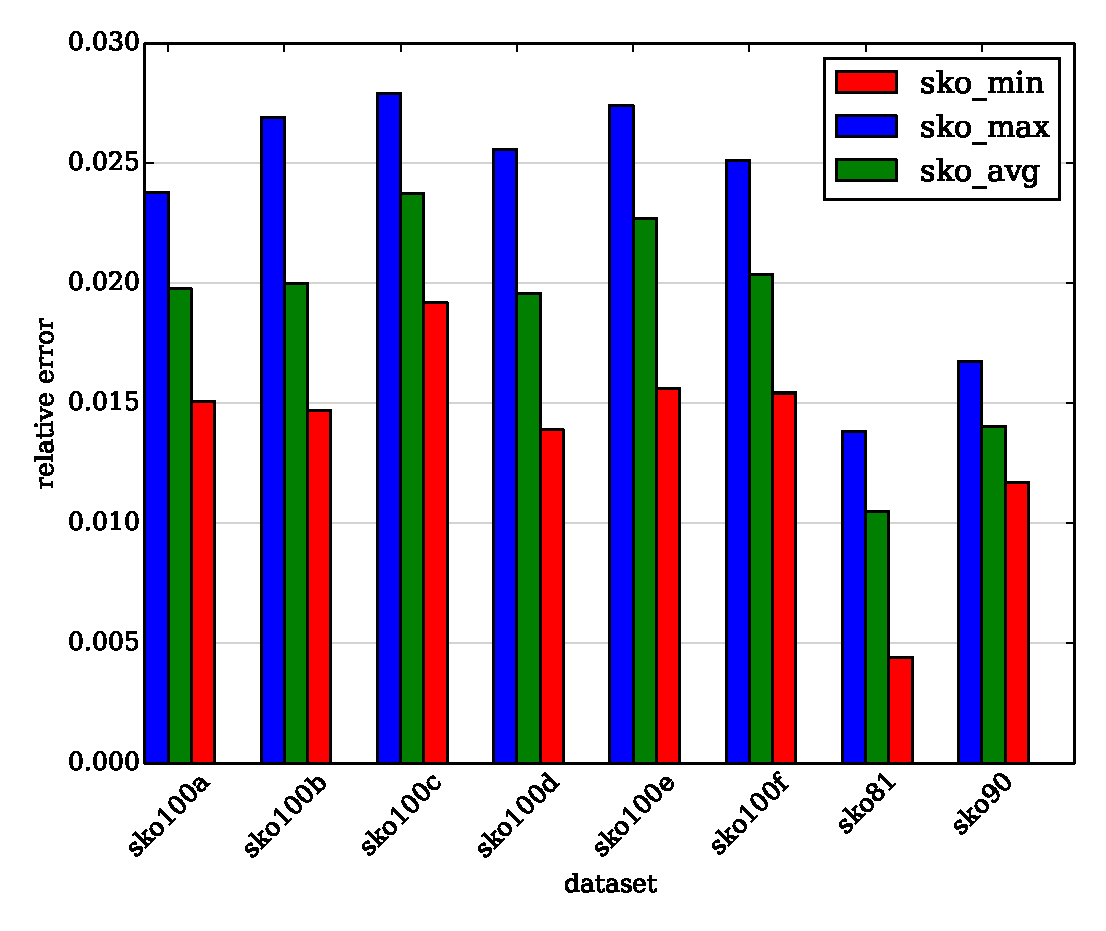
\includegraphics[width=0.9\textwidth]{algorithm/metaheuristic/charts/tsp/final/distance.eps}

  \caption{Aggregated results for various TSP instances}
  \label{figure:tsp_final}
\end{figure}

In the end it can be seen, that can be seen that proposed algorithm behaves quite well on multiple datasets, yielding results at most $10\%$ worse than optimal tours, however on some datasets approximated tour are far from optimal and cannot be considered useful. Some further work is needed in order to make use of Physarum-based Metaheuristic for reliable approximation of TSP tours.


% \input{"chapters/appendices/test_results.tex"}

% Bibliography (books, articles) starts here.
\bibliographystyle{alpha}{\raggedright\sloppy\small\bibliography{bibliography}}

% Colophon is a place where you should let others know about copyrights etc.
\cleardoublepage\ppcolophon

\end{document}
